
\chapter{Analyse et spécification des besoins}
% Une section

% Exemple d'une section qui porte une référence à une bibliographie
% NB: il faut bien suivre le syntaxe pour ne pas tomber dans le cas où il y a une référence dans la table des matières.

\section*{Introduction}

Dans ce chapitre, nous allons présenter les besoins fonctionnels et non fonctionnels, le backlog du produit et l'équipe Scrum. Ensuite, nous identifierons le diagramme de classe.
\section{Spécification des besoins} 
Dans cette partie, nous présenterons les objectifs de notre application, ce qui nous amène à identifier les acteurs du système et les besoins fonctionnels.
\subsection{Identification des acteurs}
\begin{itemize}
   

 \item \textbf{Administrateur de l'application: }L'administrateur de l'application gère les droits d'accès à l'application, consulte l'historique des modifications, effectue la création des affectations d'équipements et gère les bons d'achat et les fournisseurs. 
 \item \textbf{Utilisateur de l'application: }L'utilisateur de l'application fait partie du groupe IT et son rôle principal est de gérer les affectations d'équipements, de suivre les missions, de gérer les bons d'achat et les fournisseurs.
 \end{itemize}

\subsection{Profils utilisateurs et responsabilités}

L'identification des acteurs ne se limite pas à la distinction entre administrateur et utilisateur. Dans le contexte réel d'ASTEELFLASH, chaque profil possède un périmètre d'action précis afin de garantir la sécurité des données et la cohérence des opérations réalisées sur le parc informatique.

\begin{longtable}{|m{3.5cm}|m{5cm}|m{5cm}|}
\hline
\textbf{Profil} & \textbf{Responsabilités principales} & \textbf{Contraintes d'accès} \\
\hline
\endhead
\endfoot
\endlastfoot
\hline
Administrateur & Paramétrage des droits, consultation de l'historique, gestion complète des utilisateurs, équipements, commandes et fournisseurs & Accès complet aux fonctionnalités sensibles et aux journaux d'audit \\
\hline
Utilisateur IT & Gestion opérationnelle des équipements, affectations, missions, commandes et fournisseurs & Accès limité aux opérations métier sans modification des droits utilisateurs \\
\hline
Employé bénéficiaire & Réception ou restitution d'un équipement, consultation indirecte via les notifications reçues & Aucun accès direct à l'application dans la version actuelle \\
\hline
Product Owner & Validation fonctionnelle, priorisation du backlog, recette des modules livrés & Intervention lors des réunions de cadrage et de validation \\
\hline
\captionsetup{justification=centering,margin=1cm}
\caption{Profils utilisateurs et responsabilités associées}
\end{longtable}

Cette répartition permet d'appliquer le principe du moindre privilège : chaque utilisateur dispose uniquement des droits nécessaires à l'exécution de ses tâches.

\subsection{ Besoins fonctionnels des acteurs}
Dans cette partie, nous exposons l’ensemble des besoins fonctionnels des acteurs.
\begin{itemize}
    

   \item [$-$] \textbf{Administrateur:} 
    \begin{itemize}[label=\textbullet,font=\normalsize]
            \item Gérer les utilisateurs et leurs rôles.
            \item Gérer la gestion Matériels (équipements)
            \item Gérer les Affectations des équipements aux employés
            \item Gérer les Mission des équipements 
            \item Gérer les Bon d’achats des équipements
            \item Gérer les Fournisseurs des équipements
            \item Gérer les suivis des statistiques des équipements
            \item Gérer les Maintenances des équipements
            \item Gérer les suivis des inventaires des équipements
            \item Consulter les historiques
            \item Consulter les informations des employés
            \end{itemize}
    \newpage

    \item [$-$]\textbf{Utilisateur:}
            \begin{itemize}[label=\textbullet,font=\normalsize]
            \item Gérer la gestion des Matériels (équipements)
            \item Gérer les Affectations des équipements aux employés
            \item Gérer les Mission des équipements 
            \item Gérer les Bon d’achats des équipements
            \item Gérer les Fournisseurs des équipements
            \item Gérer les suivis des statistiques des équipements
            \item Gérer les Maintenances des équipements
            \item Gérer les suivis des inventaires des équipements
            \item Consulter les informations des employés
            \end{itemize}
\end{itemize}
   
    \subsection{Besoin non fonctionnel}
Dans cette partie, nous exposons l’ensemble des besoins non fonctionnels désignant les contraintes auxquelles est soumis le système pour son fonctionnement.

    \begin{itemize}[label=\textbullet,font=\normalsize]
    
        \item \textbf{Extensibilit\'{e} :} L'application doit \^{e}tre con\c{c}ue selon une architecture modulaire, permettant l'ajout de nouvelles fonctionnalit\'{e}s ult\'{e}rieurement sans modification majeure du code existant. Cette extensibilit\'{e} est essentielle pour accompagner l'\'{e}volution des besoins d'ASTEELFLASH et l'int\'{e}gration future de nouveaux modules tels que la gestion des licences logicielles ou le monitoring r\'{e}seau.
        
        \item \textbf{Performance :} L'application doit offrir des temps de r\'{e}ponse rapides pour garantir une exp\'{e}rience utilisateur fluide. Le temps de chargement des pages ne doit pas d\'{e}passer 3 secondes, m\^{e}me lors de la manipulation de grandes quantit\'{e}s de donn\'{e}es. Les requ\^{e}tes de recherche et de filtrage dans les listes d'\'{e}quipements doivent s'ex\'{e}cuter en moins de 2 secondes.
        
        \item \textbf{Ergonomie de l'interface :} Les interfaces doivent \^{e}tre claires, lisibles et faciles \`{a} utiliser, m\^{e}me pour des utilisateurs non techniques. Les tableaux doivent \^{e}tre bien organis\'{e}s avec une pagination, des fonctionnalit\'{e}s de tri et de recherche. La navigation doit \^{e}tre intuitive avec un menu structur\'{e} et des ic\^{o}nes explicites. Les formulaires doivent int\'{e}grer une validation c\^{o}t\'{e} client pour guider l'utilisateur.
        
        \item \textbf{Portabilit\'{e} de l'application :} L'application doit \^{e}tre accessible depuis diff\'{e}rents types de terminaux (ordinateurs de bureau, ordinateurs portables, tablettes) et compatible avec les principaux navigateurs web (Google Chrome, Mozilla Firefox, Microsoft Edge). L'interface doit s'adapter automatiquement \`{a} la r\'{e}solution de l'\'{e}cran gr\^{a}ce \`{a} un design responsive.
        
        \item \textbf{Confidentialit\'{e} et s\'{e}curit\'{e} :} Les informations disponibles \`{a} travers l'application doivent \^{e}tre confidentielles et accessibles uniquement par les personnes autoris\'{e}es. L'authentification via LDAP et Active Directory garantit que seuls les membres du groupe IT d'ASTEELFLASH peuvent acc\'{e}der \`{a} l'application. Les mots de passe ne doivent jamais \^{e}tre stock\'{e}s en clair dans la base de donn\'{e}es.

        \item \textbf{Disponibilit\'{e} :} L'application doit \^{e}tre disponible pendant les heures de travail de l'entreprise (3 postes, 40 heures/semaine). Le taux de disponibilit\'{e} vis\'{e} est de 99\% durant les heures ouvr\'{e}es. En cas de panne, le temps de r\'{e}tablissement du service ne doit pas exc\'{e}der 30 minutes.

        \item \textbf{Maintenabilit\'{e} :} Le code source doit \^{e}tre bien structur\'{e}, document\'{e} et respecter les conventions de nommage du framework ASP.NET Core. L'architecture MVC facilite la s\'{e}paration des responsabilit\'{e}s et permet une maintenance ais\'{e}e. Les configurations (cha\^{i}nes de connexion, param\`{e}tres SMTP, seuils d'alertes) doivent \^{e}tre externalis\'{e}es dans des fichiers de configuration.

        \item \textbf{Tra\c{c}abilit\'{e} :} Toutes les op\'{e}rations sensibles (ajout, modification, suppression d'\'{e}quipements, affectations, missions) doivent \^{e}tre enregistr\'{e}es dans un historique d\'{e}taill\'{e}, incluant la date, l'heure, l'utilisateur concern\'{e} et la nature de l'op\'{e}ration. Cette tra\c{c}abilit\'{e} est essentielle pour l'audit et le suivi des changements.

        \end{itemize}

\subsection{Règles métier principales}

Les règles métier définissent les conditions que l'application doit respecter pour garantir la cohérence des données et la conformité avec les procédures internes du département IT.

\begin{longtable}{|m{1.5cm}|m{5cm}|m{7.5cm}|}
\hline
\textbf{Code} & \textbf{Règle métier} & \textbf{Description} \\
\hline
\endhead
\endfoot
\endlastfoot
\hline
RM01 & Unicité de l'équipement & Chaque équipement doit être identifié par un numéro de série ou une référence unique afin d'éviter les doublons dans l'inventaire. \\
\hline
RM02 & Équipement disponible avant affectation & Un équipement ne peut être affecté à un employé que si son état est disponible et s'il n'est pas déjà affecté ou en mission. \\
\hline
RM03 & Historisation automatique & Toute création, modification ou suppression d'une donnée sensible doit générer une entrée dans l'historique. \\
\hline
RM04 & Seuil de stock minimum & Lorsque le stock disponible d'une catégorie d'équipement devient inférieur au seuil défini, un e-mail d'alerte doit être envoyé aux responsables. \\
\hline
RM05 & Mission temporaire bornée & Une mission doit posséder une date de début et une date de fin. La date de fin doit être supérieure ou égale à la date de début. \\
\hline
RM06 & Contrôle des droits & Les fonctionnalités d'administration ne sont accessibles qu'aux utilisateurs appartenant au groupe Active Directory autorisé. \\
\hline
RM07 & Suppression contrôlée & La suppression d'un équipement lié à des historiques, affectations ou commandes doit être contrôlée afin de préserver la traçabilité. \\
\hline
\captionsetup{justification=centering,margin=1cm}
\caption{Règles métier de l'application}
\end{longtable}

\subsection{Critères d'acceptation globaux}

Pour chaque fonctionnalité majeure, des critères d'acceptation ont été définis. Ils constituent une base de validation avec le Product Owner et permettent de vérifier que le résultat livré correspond bien au besoin exprimé.

\begin{longtable}{|m{4cm}|m{9cm}|}
\hline
\textbf{Fonctionnalité} & \textbf{Critères d'acceptation} \\
\hline
\endhead
\endfoot
\endlastfoot
\hline
Authentification & L'utilisateur peut se connecter avec ses identifiants Active Directory ; un message explicite apparaît en cas d'échec ; les utilisateurs non membres du groupe autorisé sont refusés. \\
\hline
Gestion des équipements & L'utilisateur peut créer, modifier, consulter, rechercher et supprimer un équipement ; les champs obligatoires sont contrôlés ; les doublons sont évités. \\
\hline
Gestion des affectations & Une affectation ne peut concerner qu'un équipement disponible ; l'employé concerné est clairement identifié ; l'historique est mis à jour automatiquement. \\
\hline
Gestion des missions & Une mission possède une durée définie ; le système permet la modification et la suppression ; un rappel est envoyé à l'échéance prévue. \\
\hline
Tableau de bord & Les indicateurs affichent la répartition des équipements par type, état et disponibilité ; les données se mettent à jour après les opérations principales. \\
\hline
Gestion des commandes & Les bons d'achat sont liés aux fournisseurs ; les détails de réception sont conservés ; les informations restent consultables dans l'historique. \\
\hline
\captionsetup{justification=centering,margin=1cm}
\caption{Critères d'acceptation des fonctionnalités principales}
\end{longtable}

\section{Diagramme de cas d’utilisation global}
La figure 2.1 représente  le diagramme de cas d'utilisation global.

Avant de présenter le diagramme, nous pouvons regrouper les cas d'utilisation selon les modules fonctionnels suivants :

\begin{itemize}[label=\textbullet,font=\normalsize]
    \item \textbf{Module sécurité :} authentification LDAP, contrôle du rôle et consultation des utilisateurs autorisés.
    \item \textbf{Module parc informatique :} gestion des équipements, consultation de l'inventaire, suivi du stock et visualisation des statistiques.
    \item \textbf{Module mouvements :} gestion des affectations, missions temporaires, retours et rappels automatiques.
    \item \textbf{Module achats :} gestion des fournisseurs, bons d'achat et réceptions.
    \item \textbf{Module audit :} consultation des historiques et suivi des actions réalisées par les utilisateurs.
\end{itemize}

Cette décomposition facilite la lecture du diagramme global et prépare la conception détaillée de chaque sprint.
 \newpage  
    
 \begin{figure}[h!]
    \centering
    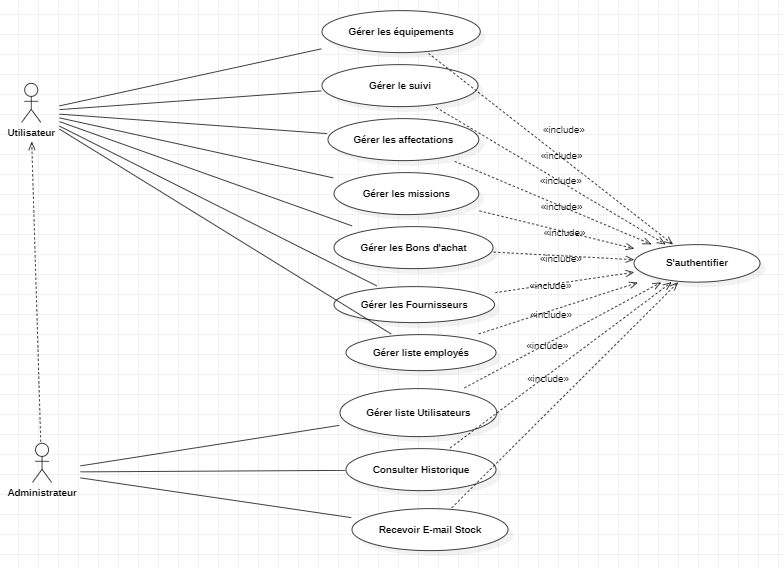
\includegraphics{img/utilisationGlobal.png}\\[1cm]
     \caption{Diagramme de Cas D'utilisation Global}
    \end{figure}\

\section{Diagramme de Classe}
Le diagramme de classes décrit la perspective structurelle d'un système en illustrant les objets au sein du système, les relations entre ces objets et les attributs et opérations associés à chaque classe d'objets. La figure 2.2 illustre le diagramme de classe global:
\newpage
\begin{figure}[h!]
    \centering
    
\includegraphics[scale=0.7]{ClassGlobal.png}\\[1cm]
     \caption{Diagramme de Classe Global}
    \end{figure}\

\section{Planification " Scrum"}    

Dans cette section, nous allons aborder le pilotage du projet par la méthodologie Scrum. Comme nous l'avons déjà mentionné, nous avons choisi Scrum en raison de sa capacité à permettre un développement rapide et la réutilisabilité des fonctionnalités indépendamment de la plateforme. Cette méthode favorise la collaboration entre différents intervenants. Dans le contexte de notre projet, notre équipe Scrum est composée de :
\begin{itemize}
    \item Product Owner: M. Wael KAOUCH 
    \item Scrum Master: Nour El Islem Jabnoun
    \item Équipe de développement : Mohamed NASRAOUI et l’équipe traçabilité
\end{itemize}



\subsection{Planification des sprints}

Pour bien organiser notre travail, nous avons besoin de diviser les tâches à effectuer en des sprints. Les sprints sont des périodes d’un mois au maximum, au bout de laquelle nous délivrons un incrément du produit, potentiellement livrable. La figure 2.3 représente la répartition des sprints:

        \begin{figure}[h!]
        \centering
        
\includegraphics[scale=0.7]{sprint.png}\\[1cm]
         \caption{Planification des Sprints}
        \end{figure}\

    \subsection{Le Planning}

  Dans la figure 2.4 présente notre planification de chaque sprint.
    
        \begin{figure}[h!]
        \centering
        
\includegraphics[scale=0.7]{planning.png}\\[1cm]
         \caption{Planning du déroulement du projet}
        \end{figure}\

    \section{Backlog Produit}
Le tableau 2.1 présente le backlog du produit de notre projet, qui détaille les différentes user stories. Il est important de souligner que le backlog du produit est un outil essentiel pour la planification et la gestion des exigences, car il regroupe toutes les fonctionnalités et les tâches à réaliser pour le produit.

        \begin{longtable}{|m{1cm}|m{3cm}|m{1cm}|m{8cm}|m{3cm}|}
                
                \hline 
                    \textbf{Id} & \textbf{Sprint}& \textbf{Id} & \textbf{Fonctionnalités}& \textbf{Priorité}\\
                \hline
                \endhead
                \endfoot
                \endlastfoot
                \hline
                \multirow{2}{*}{1} & \multirow{2}{*}{\begin{tabular}[c]{@{}c@{}}Sprint N1 : \\ Authentification et \\ gestion de profil\end{tabular}} & 1.1 & En tant qu’Administrateur ou membre de groupe IT je veux m'authentifier pour accéder à l'application. & Elevé \\
                \cline{3-5}
                 &  & 1.2 & En tant qu’Administrateur je veux gérer la liste des utilisateurs et leurs rôles. & Moyenne \\
                \hline
                \multirow{2}{*}{2} & \multirow{2}{*}{\begin{tabular}[c]{@{}c@{}}Sprint N2 : \\ Gestion des \\ équipements \\ et Gestion des \\ suivis\end{tabular}} & 2.1 & En tant qu’Administrateur ou membre de groupe IT je veux Ajouter, modifier, consulter les Détails et supprimer des équipements. & Elevé \\
                \cline{3-5}
                 &  & 2.2 & En tant qu’Administrateur ou membre de groupe IT je veux suivre les statistiques des équipements du parc informatique. & Elevé \\
                 \cline{3-5}
                 &  & 2.3 & En tant qu’Administrateur ou membre de groupe IT je veux consulter la liste des équipements du parc informatique. & Elevé \\
                 \hline       
                 \multirow{2}{*}{3} & \multirow{2}{*}{\begin{tabular}[c]{@{}c@{}}Sprint N3 : \\ Maintenance des \\ équipements\end{tabular}} & 3.1 & En tant qu’Administrateur ou membre de groupe IT je veux Ajouter, Modifier, consulter les Détails et supprimer des Affectations des équipements à l’employés. & Elevé \\
                \cline{3-5}
                 &  & 3.2 & En tant qu’Administrateur ou membre de groupe It je veux Ajouter, Modifier, consulter les Détails et supprimer les missions des équipements.
                 Un email sera transmis automatiquement à l’employé chaque fin de mission pour récupérer le matériel emprunté. & Elevé \\
                 \cline{3-5}
                 &  & 3.3 & En tant qu’Administrateur je veux suivre les historiques des équipements, des missions, des fournisseurs, réception des demandes et historique des employés. & Moyenne \\
                 \cline{3-5}
                 &  & 3.4 & En tant qu’Administrateur je veux recevoir un email d’alertes si le stock d’équipements < 4 & Moyenne \\
                 \hline
                 
                 \multirow{2}{*}{4} & \multirow{2}{*}{\begin{tabular}[c]{@{}c@{}}Sprint N4 : \\ Gestion de \\ réception des \\ Commandes \end{tabular}} & 4.1 & En tant qu’Administrateur ou membre de groupe IT je veux ajouter, Modifier, consulter les détails et supprimer la réception des demandes des Matériels  & Elevé \\
                \cline{3-5}
                 &  & 4.2 & En tant qu’Administrateur ou membre de groupe IT je veux ajouter, modifier, consulter les Détails et supprimer les fournisseurs. & Elevé \\
                 \cline{3-5}
                 &  & 4.3 & En tant qu’Administrateur ou membre de groupe IT je veux mettre à jour la liste des employés et détails et Modifier leurs données. & Moyenne \\
                 \hline       
                    
            
                
                 
              \captionsetup{justification=centering,margin=2cm}    
              \caption{Backlog Général du Produit}

            \end{longtable}

\subsection{Matrice de traçabilité des besoins}

La matrice de traçabilité permet de relier les besoins exprimés aux sprints dans lesquels ils sont pris en charge. Elle permet également de vérifier qu'aucune exigence importante n'a été oubliée durant la planification.

\begin{longtable}{|m{2cm}|m{5.5cm}|m{3cm}|m{3cm}|}
\hline
\textbf{Réf.} & \textbf{Besoin} & \textbf{Sprint} & \textbf{Type} \\
\hline
\endhead
\endfoot
\endlastfoot
\hline
BF01 & Authentification des utilisateurs par LDAP & Sprint 1 & Fonctionnel \\
\hline
BF02 & Gestion des utilisateurs et des rôles & Sprint 1 & Fonctionnel \\
\hline
BF03 & Gestion complète des équipements & Sprint 2 & Fonctionnel \\
\hline
BF04 & Consultation des statistiques et du stock & Sprint 2 & Fonctionnel \\
\hline
BF05 & Gestion des affectations aux employés & Sprint 3 & Fonctionnel \\
\hline
BF06 & Gestion des missions temporaires et rappels & Sprint 3 & Fonctionnel \\
\hline
BF07 & Consultation des historiques & Sprint 3 & Fonctionnel \\
\hline
BF08 & Gestion des fournisseurs et bons d'achat & Sprint 4 & Fonctionnel \\
\hline
BNF01 & Sécurité et confidentialité des données & Tous les sprints & Non fonctionnel \\
\hline
BNF02 & Performance et temps de réponse & Sprints 2 à 4 & Non fonctionnel \\
\hline
BNF03 & Maintenabilité et extensibilité & Tous les sprints & Non fonctionnel \\
\hline
\captionsetup{justification=centering,margin=1cm}
\caption{Matrice de traçabilité des besoins}
\end{longtable}

\subsection{Priorisation des exigences}

La priorisation des exigences a été réalisée selon la valeur métier, la criticité opérationnelle et les dépendances techniques. L'authentification a été placée en premier car elle conditionne l'accès à tous les autres modules. La gestion des équipements et du stock a ensuite été priorisée, car elle constitue le coeur de la CMDB. Les affectations, missions, commandes et fournisseurs ont été planifiés dans les sprints suivants pour compléter progressivement le cycle de vie de l'équipement.

Cette priorisation a permis de sécuriser les fonctionnalités indispensables dès les premiers incréments et de réduire les risques du projet. Elle a également facilité la validation par le Product Owner, qui pouvait évaluer l'application à chaque étape au lieu d'attendre la fin du développement.

    \section{Conclusion}
Dans ce chapitre, nous avons d\'{e}fini de mani\`{e}re d\'{e}taill\'{e}e les sp\'{e}cifications du syst\`{e}me \`{a} d\'{e}velopper. Nous avons identifi\'{e} les deux cat\'{e}gories d'acteurs (Administrateur et Utilisateur IT) et d\'{e}crit leurs besoins fonctionnels respectifs. Les besoins non fonctionnels ont \'{e}t\'{e} formalis\'{e}s autour de huit crit\`{e}res essentiels : extensibilit\'{e}, performance, ergonomie, portabilit\'{e}, confidentialit\'{e}, disponibilit\'{e}, maintenabilit\'{e} et tra\c{c}abilit\'{e}.

Le diagramme de cas d'utilisation global et le diagramme de classes nous ont permis de mod\'{e}liser la structure du syst\`{e}me et les interactions entre les diff\'{e}rents modules. La planification Scrum avec la r\'{e}partition en quatre sprints et le backlog produit d\'{e}taill\'{e} constituent la feuille de route pour la r\'{e}alisation du projet.

Le prochain chapitre pr\'{e}sentera les choix technologiques, l'architecture de l'application et la r\'{e}alisation des premiers sprints.

